\begin{priprava}{3}{}{Mere osredinjenosti}{Osnove statistike}{frontalna, delo v dvojicah/individualno}{drsnice, projekcija, računalniki}

    \section{Mere osredinjenosti}

        

    \subsubsection{Aritmetična sredina}
        \textbf{Aritmetična sredina} ali \textbf{povprečje} je količnik vsote vseh vrednosti 
        statistične spremenljivke in števila teh vrednosti. \\

        $$\overline{x}=\dfrac{x_1+x_2+\cdots+x_n}{N}=\dfrac{1}{N}\sum_{i=1}^n x_i.$$
    %                 
    % 
        Če se vrednosti statistične spremenljivke ponavljajo ($k_i$ vrednosti $x_i$), je formula sledeča:
        $$\overline{x}=\dfrac{k_1x_1+k_2x_2+\cdots+k_mx_m}{k_1+k_2+\cdots+k_m}=\dfrac{\sum_{i=1}^mk_ix_i}{\sum_{i=1}^mk_i}; \quad \sum_{i=1}^mk_i=N$$

       

    
        Pri grupiranih podatkih za vrednosti vzamemo sredine frekvenčnih razredov.
    




    \subsubsection{Modus}
        \textbf{Modus} ali \textbf{gostiščnica $Mo$} je vrednost statistične spremenljivke, ki se v množici vseh vrednosti najpogosteje ponavlja.                 
    
            ~
    
        Če se v neki množici dve vrednosti pojavita enako mnogokrat najpogosteje, rečemo, da je porazdelitev vrednosti \textbf{bimodalna}.
    

    
        Za grupirane podatke določamo \textbf{modalni razred}, to je tisti razred, ki ima največjo frekvenčno gostoto.
    



    \subsubsection{Mediana}
        \textbf{Mediana} ali \textbf{središčnica $Me$} je tista vrednost statistične spremenljivke, pri kateri je polovica vrednosti večjih ali enakih,
        druga polovica vrednosti pa manjših ali enakih od te vrednosti.                 
    
            ~
    
        Če imamo liho število vrednosti statistične spremenljivke, za mediano vzamemo vrednost, ki stoji na mestu $\frac{n+1}{2}$ po velikosti urejenih podatkov. \\
        Če je število vrednosti sodo, za vrednost mediane vzamemo aritmetično sredino srednjih dveh podatkov.
    


    \subsubsection{Kvartili}

    
        Mediana razdeli podatke na dve polovici. Ti dve polovici lahko spet razdelimo na dve polovici in dobimo štiri enako močne množice podatkov. 
        Meje teh skupin imenujemo \textbf{kvartili}.
    
            ~


        \textbf{Prvi kvartil $Q_1$} je mediana prve (spodnje) polovice podatkov, \textbf{drugi kvartil $Q_2$} je mediana $Me$ vseh podatkov,
        \textbf{tretji kvartil $Q_3$} pa je mediana druge (zgornje) polovice podatkov.
    
            ~
    
        Vrednosti kvartilov, minimalno vrednost in maksimalno vrednost množice podatkov grafično predstavimo
         z \textbf{diagramom kvartilov} oziroma \textbf{šktalo z brki}. \\~

        \begin{figure}[H]
        \centering
         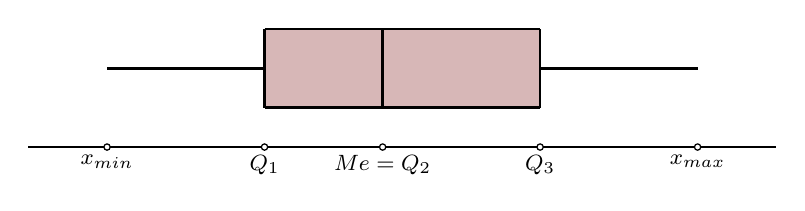
\begin{tikzpicture}
            % \clip (0,0) rectangle (14.000000,10.000000);
            {\footnotesize
            
            % Marking point x_{min} by circle
            \draw [line width=0.016cm] (1.500000,1.000000) circle (0.040000);%
            \draw (1.500000,1.000000) node [anchor=north] { $x_{min}$ };%
            
            % Marking point Q_1 by circle
            \draw [line width=0.016cm] (3.500000,1.000000) circle (0.040000);%
            \draw (3.500000,1.000000) node [anchor=north] { $Q_1$ };%
            
            % Marking point Me=Q_2 by circle
            \draw [line width=0.016cm] (5.000000,1.000000) circle (0.040000);%
            \draw (5.000000,1.000000) node [anchor=north] { $Me=Q_2$ };%
            
            % Marking point Q_3 by circle
            \draw [line width=0.016cm] (7.000000,1.000000) circle (0.040000);%
            \draw (7.000000,1.000000) node [anchor=north] { $Q_3$ };%
            
            % Marking point x_{max} by circle
            \draw [line width=0.016cm] (9.000000,1.000000) circle (0.040000);%
            \draw (9.000000,1.000000) node [anchor=north] { $x_{max}$ };%
            
            % Drawing segment a b
            \draw [line width=0.016cm] (0.500000,1.000000) -- (1.460000,1.000000);%
            \draw [line width=0.016cm] (1.540000,1.000000) -- (3.460000,1.000000);%
            \draw [line width=0.016cm] (3.540000,1.000000) -- (4.960000,1.000000);%
            \draw [line width=0.016cm] (5.040000,1.000000) -- (6.960000,1.000000);%
            \draw [line width=0.016cm] (7.040000,1.000000) -- (8.960000,1.000000);%
            \draw [line width=0.016cm] (9.040000,1.000000) -- (10.000000,1.000000);%
            
            % Changing color 215 183 183
            \definecolor{r215g183b183}{rgb}{0.843137,0.717647,0.717647}%
            \color{r215g183b183}% 
            
            % Filling rectangle left-bottom: f right-top: i
            \fill (3.500000,2.500000) -- (7.000000,2.500000) -- (7.000000,1.500000) -- (3.500000,1.500000);%
            
            % Changing color 0 0 0
            \definecolor{r0g0b0}{rgb}{0.000000,0.000000,0.000000}%
            \color{r0g0b0}% 
            
            % Drawing segment c d
            \draw [line width=0.032cm] (1.500000,2.000000) -- (3.500000,2.000000);%
            
            % Drawing segment e f
            \draw [line width=0.032cm] (3.500000,1.500000) -- (3.500000,2.500000);%
            
            % Drawing segment g h
            \draw [line width=0.032cm] (5.000000,1.500000) -- (5.000000,2.500000);%
            
            % Drawing segment i j
            \draw [line width=0.032cm] (7.000000,1.500000) -- (7.000000,2.500000);%
            
            % Drawing segment k l
            \draw [line width=0.032cm] (7.000000,2.000000) -- (9.000000,2.000000);%
            
            % Drawing segment e i
            \draw [line width=0.032cm] (3.500000,1.500000) -- (7.000000,1.500000);%
            
            % Drawing segment f j
            \draw [line width=0.032cm] (3.500000,2.500000) -- (7.000000,2.500000);%
            \color{black}
            }
            \end{tikzpicture}
        \end{figure}
    

        ~


%%%% naloge


    \begin{naloga}
        Izračunajte aritmetično sredino količin.
        \begin{itemize}
            \item $1.5~s$, $3.5~s$, $1~s$
            \item $4~km$, $2000~m$, $3~km$
            \item $4~€$, $2~€$, $3~€$, $1~€$, $5~€$
        \end{itemize}
    \end{naloga}

    \begin{naloga}
        Izračunajte aritmetično sredino danim podatkom.
        \begin{itemize}
            \item $2, 3, 1, 8, 19, 2, 7$
            \item $13, 39, 12$
            \item $0.3, 0.4, 0.5, 0.7, 0.6$
        \end{itemize}            \end{naloga}



    \begin{naloga}
        Določite modus danim številskim podatkom.
        \begin{itemize}
            \item $1, 4, 2, 4, 1, 6, 3, 4, 1, 4, 6, 4, 4, 8$
            \item $3, 25, 10, 3, 5, 7, 5, 7, 9, 4, 49$
            \item $\dfrac{1}{3}, \dfrac{3}{4}, \dfrac{1}{2}, \dfrac{6}{8}, \dfrac{2}{9}$
            \item $\dfrac{1}{2}, \dfrac{2}{4}, \dfrac{1}{4}, \dfrac{5}{10}, \dfrac{8}{9}$
        \end{itemize}
    \end{naloga}

    \begin{naloga}
        V porodnišnici so izmerili dolžine dojenčkov, ki so se rodili v enem dnevu.  \\
        $50, 51, 51, 44, 47, 48, 53, 49, 52, 55, 46, 50, 50, 49, 47, 47$ \\
        Določite mediano podatkov.
    \end{naloga}





    \begin{naloga}
     
     Otroci v vrtcu so metali žogo na koš in si zapisovali dosežke. Podatki so prikazani v preglednici. 

         \begin{table}[H]
             \centering
             \begin{tabular}{||c|c|c|c|c|c|c|c|c|c||} 
             \hhline{|t:==========:t|}
             \rowcolor[rgb]{0.843,0.718,0.718} 
             Otrok  & Jaka & Jure & Miha & Polona & Valerija & Tina & Mojca & Cene & Darja   \\ 
             \hhline{|:==========:|}
             Št.~košev & $5$ & $7$ & $10$ & $8$ & $5$ & $6$ & $9$ & $9$& $4$  \\ 
             \hhline{|b:==========:b|}
             \end{tabular}
         \end{table}

        Izračunajte, koliko košev je otrok zadel v povprečju. Podatke uredite po vrsti in določite $Mo$, $Me$ ter narišite škatlo z brki.

    \end{naloga}



\end{priprava}